\documentclass{beamer}
% \usetheme[nogauge,amurmapleblue,sidebar]{Amurmaple}
\usetheme[nogauge,amurmapleblue]{Amurmaple}

\usepackage{todonotes}

\newcommand{\plugin}[1]{\texttt{#1}}

\title{Let's SCIP it!}
\author{Author Name}
\titlegraphic{
\includegraphics[width=3.5cm]{sciplogo.png}}
% \logo{\hspace{1mm}\includegraphics[width=1.8cm]{newscippy.png}}
\logo{\hspace{1mm}
\includegraphics[width=1.8cm]{sciplogo.png}}

\begin{document}

\begin{frame}
  \maketitle
\end{frame}

\section{Out-of-the-box Solver}

\begin{frame}{SCIP as a Black-Box Solver}
  \begin{itemize}
  \item SCIP is a solver for finding globally optimal solutions of
    \begin{itemize}
    \item mixed-integer (nonlinear) programs
    \item satisfiability problems
    \item constraint integer programs
    \end{itemize}
  \item supports exact arithmetic for mixed-integer linear programs
  \end{itemize}
\end{frame}

\begin{frame}{Interfaces}
  SCIP has interfaces to many popular programming languages
  \begin{itemize}
  \item C/C++
  \item Python
  \item Julia
  \item Rust
  \item Matlab
  \item Java
  \end{itemize}
\end{frame}

\begin{frame}{SCIP is Easy to Use}
  \begin{itemize}
  \item executable can read many popular file formats (mps, lp, etc.)
  \item modeling problems via SCIP's interfaces is very easy
  \end{itemize}
  \missingfigure{Add some Python code here.}
\end{frame}

\sepframe[title={Branch-and-Price},image={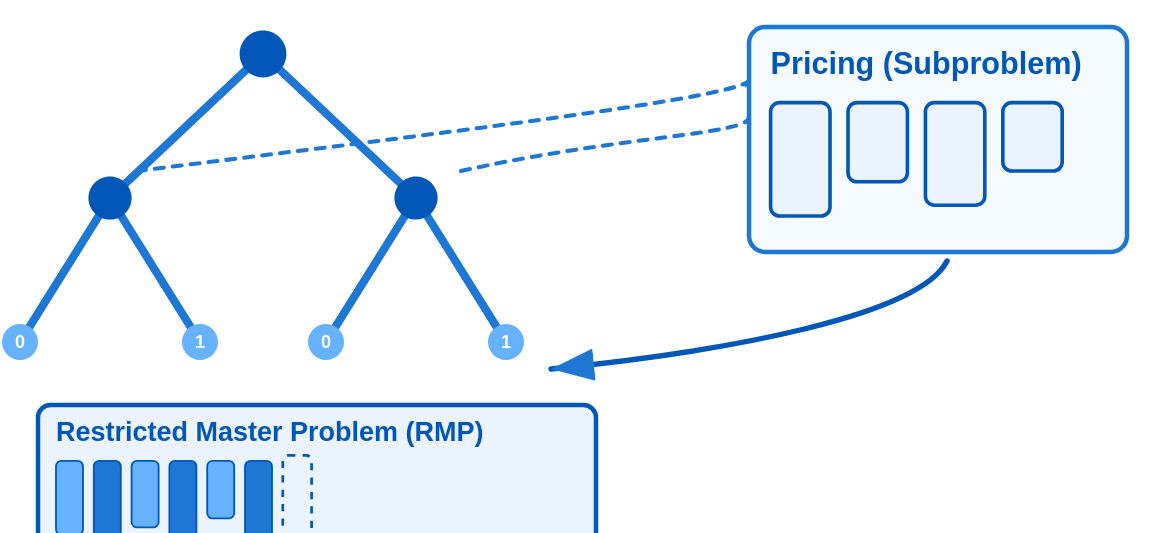
\includegraphics[width=6cm]{scip-bap.png}}]

\section{Branch-and-Price}

\begin{frame}{Branch-and-Price}
  required functionality
  \begin{itemize}
  \item column generation
  \item embedding of column generation in branch-and-bound
  \item custom branching rules
  \end{itemize}

  \vfill

  SCIP naturally supports these features by
  \begin{itemize}
  \item plugin for generating new columns (\plugin{pricer})
  \item automatic handling of branch-and-bound tree including warm start and heuristics
  \item plugin for custom branching rules (\plugin{branching rule})
  \end{itemize}

  \vfill
\end{frame}

\section{Custom Bounds}

\begin{frame}{Custom Bounds}
  required functionality
  \begin{itemize}
  \item access to variables with local bounds (modified during
    solving process)
  \item embedding of custom bound in branch-and-bound
  \end{itemize}

  \vfill
  
  SCIP naturally supports these features by
  \begin{itemize}
  \item plugin for computing custom bound (\plugin{relaxator})
  \item automatic embedding in branch-and-bound
  \end{itemize}

  \vfill
\end{frame}

\section{Separation}

\begin{frame}{Cutting Planes}
  required functionality
  \begin{itemize}
  \item access to solution
  \item creating and adding custom cutting planes
  \end{itemize}

  \vfill

  SCIP naturally supports these featurs by
  \begin{itemize}
  \item plugin for custom cutting planes (\plugin{separator})
  \item automatic embedding in branch-and-bound, including cut storage and selection
  \item full control of timing of cut generation
    \begin{itemize}
    \item only at root node
    \item every~$k$-th level of the branch-and-bound tree
    \end{itemize}
  \end{itemize}

  \vfill
\end{frame}

\section{Propagation}

\begin{frame}{Variable Bound Propagation}
  required functionality
  \begin{itemize}
  \item access to local variable bounds (during solving process)
  \item possibility to change local variable bounds
  \end{itemize}

  \vfill

  SCIP naturally supports these featurs by
  \begin{itemize}
  \item plugin for propagation methods (\plugin{propagator})
  \item automatic embedding in branch-and-bound
  \item full control of timing of propagation
    \begin{itemize}
    \item only at root node
    \item every~$k$-th level of the branch-and-bound tree
    \item before or after solving LP relaxation
    \end{itemize}
  \end{itemize}

  \vfill  
\end{frame}

\section{Presolving}

\begin{frame}{Presolving}
  required functionality
  \begin{itemize}
  \item custom rules for simplifying a problem
  \end{itemize}

  \vfill

  SCIP naturally supports these featurs by
  \begin{itemize}
  \item plugin for presolving methods (\plugin{presolver})
  \item synchronization with other presolving routines
  \item full control of presolving behavior
    \begin{itemize}
    \item maximum number of rounds
    \item classification of expected required time (fast, medium, exhaustive)
    \end{itemize}
  \end{itemize}

  \vfill
\end{frame}

\section{Heuristics}

\begin{frame}{Heuristics}
  required functionality
  \begin{itemize}
  \item access to local or global variable bounds
  \item embedding of heuristic search within branch-and-bound
  \end{itemize}

  \vfill

  SCIP naturally supports these featurs by
  \begin{itemize}
  \item plugin for heuristics (\plugin{heuristic})
  \item automatically called during solving process
  \item automatic check whether solution is feasible
  \item full control of behavior
    \begin{itemize}
    \item frequency of calling heuristic
    \item before/after solving LP, before/during/after presolving
    \end{itemize}
  \end{itemize}

  \vfill
\end{frame}

\section{Branching Rules}

\begin{frame}{Branching Rules}
  required functionality
  \begin{itemize}
  \item access to LP solution and local variable bounds
  \item add branching decision
  \end{itemize}

  \vfill

  SCIP naturally supports these featurs by
  \begin{itemize}
  \item plugin for branching rules (\plugin{branching rule})
  \item automatic embedding in branch-and-bound
  \item supports
    \begin{itemize}
    \item variable branching
    \item constraint-based branching
    \end{itemize}
  \end{itemize}

  \vfill
\end{frame}

\section{Benders Decomposition}

\begin{frame}{Benders Decomposition}
  required functionality
  \begin{itemize}
  \item access to LP or IP solution
  \item embedding of Benders cuts in branch-and-bound
  \end{itemize}

  \vfill

  SCIP naturally supports these featurs by
  \begin{itemize}
  \item plugin for custom Benders decomposition (\plugin{benders})
  \item plugin for custom Benders cuts (\plugin{benderscut})
  \item automatic embedding of Benders cuts into branch-and-bound
  \end{itemize}

  \vfill
\end{frame}

\section{Custom Constraints}

\begin{frame}{Custom Constraints}
  required functionality
  \begin{itemize}
  \item abstract mechanism to define constraints (not necessarily
    represented by linear inequalities)
  \item accept or reject solutions
  \end{itemize}

  \vfill

  SCIP naturally supports these featurs by
  \begin{itemize}
  \item plugin for custom constraints (\plugin{constraint handler})
  \item features
    \begin{itemize}
    \item mechanism to accept or reject (heuristic) solutions
    \item presolving reductions
    \item cutting plane separation
    \item propagation
    \end{itemize}
  \end{itemize}

  \vfill
\end{frame}

\begin{frame}
  You wonder how to solve mixed-integer (nonlinear) programs?

  \vfill
  \uncover<2->
  {
    \flushright \LARGE \textbf{Let's SCIP it!}
  }
\end{frame}

% \begin{frame}{}
%   required functionality
%   \begin{itemize}
%   \item 
%   \end{itemize}

%   \vfill

%   SCIP naturally supports these featurs by
%   \begin{itemize}
%   \item 
%   \end{itemize}

%   \vfill
% \end{frame}

\end{document}

%%% Local Variables:
%%% coding: utf-8
%%% mode: latex
%%% TeX-master: t
%%% End:
